We have installed a Jupyter server as a component of our MathHub system.
It provides a normal Jupyter server except for additionally supporting our MMT kernel.
It is available at the URL \url{jupyter.mathhub.info}.\ednote{@Kai: check this}

We have added Jupyter notebooks as a new document type in MathHub.info\footnote{As the MathHub front-end is currently undergoing major re-write.
  The old MathHub interface was based on Drupal, which led to major system vulnerabilities and therefore maintenance hassles, because Drupal was targeted by hackers.
  We are currently working on a docker-based orchestration of services with a React.JS based front-end in the general spirit of the OpenDreamKit VRE toolkit; see \url{https://github.com/MathHubInfo/}. The new system can be accessed at \url{http://new.mathhub.info}.}; see Figure~\ref{fig:mathhub-NB} for an example. In the MathHub front-end, documents are displayed with multiple tabs:
\begin{compactenum}
\item \textsf{view} gives a preview of the notebook, essentially the computation cells without output, pre-rendered for served static cally without a kernel.\ednote{MK: we should implement this; I am not sure what the best way is for this. I guess a build target based on \texttt{https://github.com/jendas1/jupyter-notebook-quick-look}.}
\item \textsf{run/edit} starts the respective notebook  on \url{jupyter.mathhub.info} for running and editing; any changes to the notebook are committed to the Git repository on  \url{gl.mathhub.info} that hosts the notebook. 
\item \textsf{metadata} (this is the tab open in Figure~\ref{fig:mathhub-NB}), shows the metadata provided by the Jupyter kernel and the repository. 
\item \textsf{source} provides access to the document source; here simply a link to \url{gl.mathhub.info}
\item \textsf{statistics} shows statistical information about the notebook, its ephemeral document (see Figure~\ref{fig:test_theory} and the discussion there), and the connections into the background theory graph. 
\item \textsf{graph} links to the a display of the graphs (document graph, declaration graph, and dependency graph) induced by the document and the background knowledge via TGView, a canvas-based in-browser visualizer for knowledge graph information~\cite{RupKohMue:fitgv17}.
\end{compactenum}
This integration combines the interactive features of the Jupyter server with the knowledge management facilities on MathHub.info. In the future, we plan to integrate the notebook diff/patch \textsf{nbdime} developed in OpenDreamKit to extend the knowledge management facilities. 

\begin{figure}[ht]\centering
  \fbox{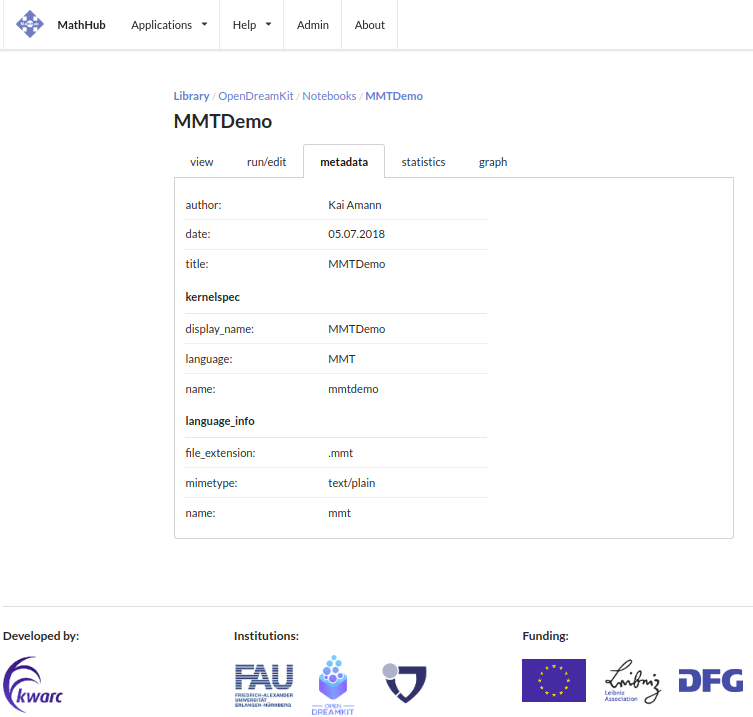
\includegraphics[width=13cm]{NB-Mathhub}}
  \caption{A Jupyter Notebook in MathHub.info (Metadata)}\label{fig:mathhub-NB}
\end{figure}

A Jupyter Notebook additionally has a special button appears that allows users to open the notebook in the associated Jupyter server. Currently these notebooks do not use the MMT process running on MathHub.info, due to the architecture of the MMT Kernel. Therefore they currnetly do not have access to the MathHub universe. \ednote{KA: if the Kernel server would run on the same VM as the MathHub MMT we could give the kernel access to it}
\ednote{@Kai, @Tom: check this, do the implementation}

\ednote{KA: write some demo notebooks stored in gl.mathhub.info, including the one corresponding to the example in the previous section}


%%% Local Variables:
%%% mode: latex
%%% mode: visual-line
%%% fill-column: 5000
%%% TeX-master: "report"
%%% End:

%  LocalWords:  Jupyter ednote
